\section{Diversidad}

Mantener la diversidad es crucial para evitar una convergencia prematura hacía un óptimo local. Rosca \cite{Rosca} concluyó que las poblaciones parecían quedar estancadas
en un óptimo local cuando la entropía no cambiaba o decrecía monótonamente en las generaciones sucesivas. En programación genética, la diversidad se refiere a diferencias estructurales, 
como por ejemplo la cantidad de genotipos distintos en la población o la singularidad de valores del fitness \cite{genetic}. Uno de los objetivos de este trabajo es investigar cómo la 
división en castas afecta a la diversidad, así que en esta sección se analizará.  Hay diferentes medidas para calcularla, entre ellas: diversidad genotípica, 
diversidad fenotípica, entropía, pseudo-isomorfismo, distancias de edición, etc. De entre ellas calcularemos la \textbf{entropía}, que describe cómo se distribuye la
población en torno a los diferentes valores del fitness, y la \textbf{distancia de edición}, en la que cada individuo se mide contra el mejor individuo encontrado hasta el 
momento. Se han elegido dado que según Burke \cite{diversity} la entropía y la distancia de edición muestran una gran correlación con el aumento y decremento del valor 
del fitness. Una vez calculadas, se investigará la relación entre el fitness y la diversidad \cite{diversity}. 

\subsection{Experimentos}

Para realizar estas pruebas usaremos la configuración de la Tabla \ref{tab:diversity_config}, como función a minimizar la función Rastrigin\cite{BBOB}, y la distancia Euclídea.

\begin{table}[]
    \centering
    \begin{tabular}{||c|c||}
        \hline
        \multicolumn{2}{|l|}{\textbf{Fichero Configuración: config\_file\_5.json}} \\ \hline
        Tamaño del cromosoma                            & 20              \\ \hline
        Tamaño de la población                          & 100             \\ \hline
        Máximo de generaciones                          & 15              \\ \hline
        Porcentaje Alfa de la población                 & 10              \\ \hline
        Porcentaje Beta de la población                 & 20              \\ \hline
        Porcentaje Gamma de la población                & 20              \\ \hline
        Porcentaje Delta de la población                & 20              \\ \hline
        Porcentaje Epsilon de la población              & 30              \\ \hline
        Ratio de mutación                               & 10              \\ \hline
    \end{tabular}
    \caption{Parámetros de configuración para exploración de la diversidad}
    \label{tab:diversity_config}
\end{table}

\begin{figure}[H]
	\centering	
	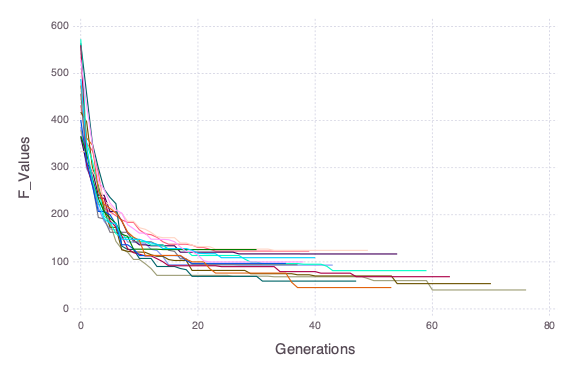
\includegraphics[scale=0.6]{figuras/config_file_5_Rastrigin.png}
	\caption{Primera ejecución}
    \label{fig:primera_ejecucion}
\end{figure}

En la Figura \ref{fig:primera_ejecucion} se ve el resultado de ejecutar el algoritmo 15 veces con la configuración anterior.
Se puede observar cómo los mejores resultados se obtienen en las primeras generaciones. La mayoría de las ejecuciones muestran cómo la mejora
del fitness disminuye alrededor de la generación 15-20. Esto puede indicar que cuanto mayor es la generación menor es la diversidad. 
Para apoyar esta idea tenemos las Figuras \ref{fig:best_f_value} y \ref{fig:worst_f_value}. 

La Figura \ref{fig:best_f_value} muestra la diversidad de la ejecución que resulta en un mejor fitness. De la generación 0 a la 30 se produce un decremento de la entropía,
pero se vuelve a recuperar en el resto de generaciones. La entropía empezando y acabando casi con el mismo valor nos dice que el algoritmo mantiene una diversidad similar a 
lo largo de toda la ejecución, lo que puede dar lugar a mejores resultados. En la Figura \ref{fig:worst_f_value}, que muestra la peor ejecución, podemos 
ver un comportamiento similar; el descenso también se produce en las generaciones 0-25. 

\begin{table}[]
    \begin{tabular}{||c|c|c|c|c|c||}
    \hline
                             & \textbf{Evals. de f} & \textbf{Entropía} & \textbf{Distancia de edición} & \textbf{Mejor f} & \textbf{Generaciones} \\ \hline
    \textbf{Mejor ejecución} & 11873                      & 2.69              & 6.20                          & 40.27                     & 77                    \\ \hline
    \textbf{Peor ejecución}  & 4900                       & 2.11              & 5.95                          & 126.14                    & 31                    \\ \hline
    \end{tabular}
    \caption{Comparación de la mejor y la peor ejecución}
    \label{fig:Comparación}
\end{table}

En ambas imágenes la distancia de edición mantiene una correlación estrecha con el valor del fitness, y en ambos casos acaba con unos valores similares. Mirando la tabla \ref{fig:Comparación}, y las figuras
mencionadas no se puede concluir una diferencia clave que marque el por qué una es la mejor ejecución y otra la peor.

\begin{figure}[]
	\centering	
	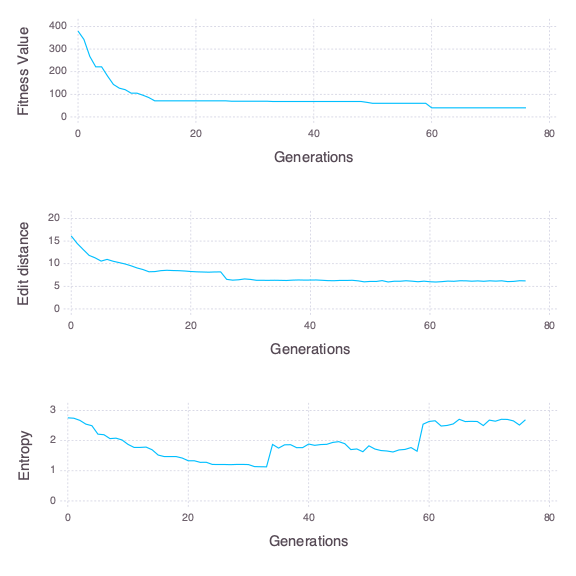
\includegraphics[scale=0.5]{figuras/config_file_5_Rastrigin_best_f_value.png}
	\caption{ Diversidad en la ejecución con mejor resultado de fitness }
    \label{fig:best_f_value}
\end{figure}

\begin{figure}[]
	\centering	
	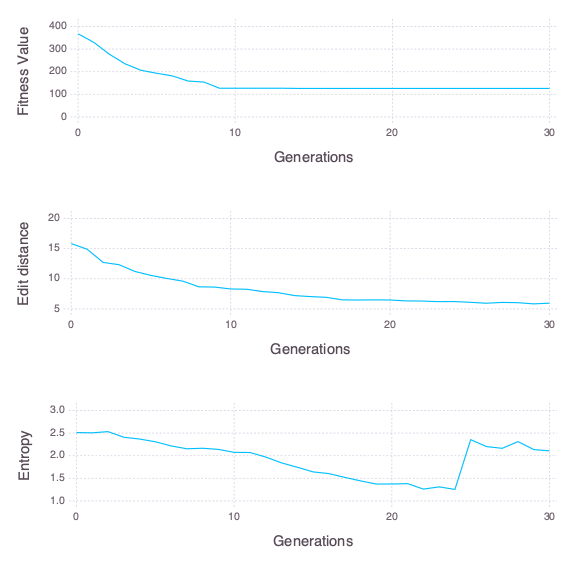
\includegraphics[scale=0.5]{figuras/config_file_5_Rastrigin_worst_f_value.png}
	\caption{ Diversidad en la ejecución con peor resultado de fitness }
    \label{fig:worst_f_value}
\end{figure}
